
\subsection{Evaluation of the convective terms}

As seen before, the discretization of the generalized convection--diffusion equations requires the values of certain variables at points different from the nodes. In this section several methods to compute $\phi$ at faces are given. The values of $\rho$ and $\Gamma$ will be assumed to be known at the nodal points. East face will be taken as reference for simplicity. The generalization to the remaining faces is straightforward. 

\subsubsection{Upwind--Difference Scheme (UDS)}

Incompressible flows and gases at low Mach number are more influenced by upstream conditions than downstream conditions. 
Let $(\vb{v} \vdot \vb{n})_e$ denote the value of the dot product $\vb{v} \vdot \vb{n}$ at east face $\cs{Pe}$. If $(\vb{v} \vdot \vb{n})_e > 0$, fluid flows from node $P$ to node $E$, hence $P$ is the upstream node and $E$ is the downstream node. Conversely, if $(\vb{v} \vdot \vb{n})_e < 0$, nodes interchange their roles as fluid flows from node $E$ to node $P$. This situation is pictured in figures \ref{fig:uds_positive_dot_product} and \ref{fig:uds_negative_dot_product}.

\begin{figure}[h]
	\centering
	\begin{minipage}{.5\textwidth}
		\centering
		\begin{tikzpicture}
			% Fill
			\fill[black!20!white] (0,0) rectangle (6,2);
			% Nodes
			\filldraw[greenNode] (1.5,1) circle (2.5pt);
			\node[greenNode, yshift=0.3cm] at (1.5,1) {$P$};
			\filldraw[greenNode] (4.5,1) circle (2.5pt);
			\node[greenNode, yshift=0.3cm] at (4.5,1) {$E$};
			% Vectors
			\draw[->, thick, blue!70!white, yshift=+0.5mm] (3,1) -- node[above]{$\vb{n}$} ++(1,0);
			\draw[->, thick, red!70!white, yshift=-0.5mm] (3,1) -- node[below]{$\vb{v}$} ++(0.75,0);
			% Control volumes
			\draw[thick] (0,0) rectangle (6,2);
			\draw[thick] (3,0) -- ++(0,2);
			\node[circle, inner sep=0pt, outer sep=0pt, black, yshift=0.5cm, fill=black!20!white] at (3,0) {$\cs{Pe}$};
		\end{tikzpicture}
		\captionsetup{width=0.9\textwidth}
		\caption{Since $(\vb{v} \vdot \vb{n})_e > 0$ fluid flows from node $P$ (upstream node) to node $E$ (downstream node).}
		\label{fig:uds_positive_dot_product}
	\end{minipage}%
	\begin{minipage}{.5\textwidth}
		\centering
		\begin{tikzpicture}
			% Fill
			\fill[black!20!white] (0,0) rectangle (6,2);
			% Nodes
			\filldraw[greenNode] (1.5,1) circle (2.5pt);
			\node[greenNode, yshift=0.3cm] at (1.5,1) {$P$};
			\filldraw[greenNode] (4.5,1) circle (2.5pt);
			\node[greenNode, yshift=0.3cm] at (4.5,1) {$E$};			
			% Vectors
			\draw[->, thick, blue!70!white] (3,1) -- node[above]{$\vb{n}$} ++(1,0);
			\draw[->, thick, red!70!white] (3,1) -- node[above]{$\vb{v}$} ++(-0.75,0);			
			% Control volumes
			\draw[thick] (0,0) rectangle (6,2);
			\draw[thick] (3,0) -- ++(0,2);
			\node[circle, inner sep=0pt, outer sep=0pt, black, yshift=0.5cm, fill=black!20!white] at (3,0) {$\cs{Pe}$};
		\end{tikzpicture}
		\captionsetup{width=0.9\textwidth}
		\caption{Since $(\vb{v} \vdot \vb{n})_e < 0$ fluid flows from node $E$ (upstream node) to node $P$ (downstream node).}
		\label{fig:uds_negative_dot_product}
	\end{minipage}
\end{figure}

\noindent
If $(\vb{v} \vdot \vb{n})_e = 0$, it implies $\vb{v}_e$ lies in the orthogonal subspace to the vector space generated by $\vb{n}$. As a result, given the approximations taken, there is no fluid flow through face $\cs{Pe}$.

The Upwind--Difference Scheme assigns $\phi_e$ the value of $\phi$ at the upstream node, that is,
\begin{equation}
	\phi_e^\text{UDS} = 
	\left\{
	\begin{aligned}
		&\phi_P & &\text{if } (\vb{v} \vdot \vb{n})_e > 0 \\
		&\phi_E & &\text{if } (\vb{v} \vdot \vb{n})_e < 0 \\
	\end{aligned}
	\right.
\end{equation}
This can be expressed in a more compact form as follows
\begin{equation}
	\dot{m}_e ( \phi_e^\text{UDS} - \phi_P ) = 
	\frac{\dot{m}_e - \abs{\dot{m}_e}}{2} ( \phi_E - \phi_P )
\end{equation}
since the approximation to compute $\dot{m}_e$ is related to $(\vb{v} \vdot \vb{n})_e$ through the relation $\dot{m}_e = (\vb{v} \vdot \vb{n})_e S_{Pe}$. The scheme is shown in figures \ref{fig:uds_upstream_node_P} and \ref{fig:uds_upstream_node_E}.

\begin{figure}[h]
	\centering
	\begin{minipage}{.5\textwidth}
		\centering
		\begin{tikzpicture}
			% Ground
			\draw[thick] (0,0) -- ++(6,0);
			% Point P
			\filldraw[black] (0.5,0) circle (2pt);
			\draw[dashed] (0.5,0) -- ++(0,1.5);
			\node[black, yshift=-0.5cm] at (0.5,0) {$P$};
			\filldraw[blue!70!white] (0.5,1.5) circle (2pt);
			\node[blue, yshift=0.5cm] at (0.5,1.5) {$\phi_P$};
			% Point e
			\filldraw[black] (2.5,0) circle (2pt);
			\draw[dashed] (2.5,0) -- ++(0,1.5);
			\node[black, yshift=-0.5cm] at (2.5,0) {$e$};
			\filldraw[blue!70!white] (2.5,1.5) circle (2pt);
			\node[blue, yshift=0.5cm] at (2.5,1.5) {$\phi_e$}; 
			% Point E
			\filldraw[black] (5.5,0) circle (2pt);
			\draw[dashed] (5.5,0) -- ++(0,3);
			\node[black, yshift=-0.5cm] at (5.5,0) {$E$};
			\filldraw[blue!70!white] (5.5,3.0) circle (2pt);
			\node[blue, yshift=0.5cm] at (5.5,3.0) {$\phi_E$};
			% Blue line
			\begin{scope}[very thick,decoration={
					markings,
					mark=at position 0.5 with {\arrow{>}}}
				] 
				\draw[thick, blue!70!white, postaction={decorate}] (0.5,1.5) -- ++(2,0);
			\end{scope}
			% Mass flow
			\draw[->, red, thick] (1.75,0.75) -- ++(1.5,0) node[above]{$\dot{m}_e > 0$};
		\end{tikzpicture}
		\captionsetup{width=0.9\textwidth}
		\caption{UDS when $(\vb{v} \vdot \vb{n})_e > 0$.}
		\label{fig:uds_upstream_node_P}
	\end{minipage}%
	\begin{minipage}{.5\textwidth}
		\centering
		\begin{tikzpicture}
			% Ground
			\draw[thick] (0,0) -- ++(6,0);
			% Point P
			\filldraw[black] (0.5,0) circle (2pt);
			\draw[dashed] (0.5,0) -- ++(0,1.5);
			\node[black, yshift=-0.5cm] at (0.5,0) {$P$};
			\filldraw[blue!70!white] (0.5,1.5) circle (2pt);
			\node[blue, yshift=0.5cm] at (0.5,1.5) {$\phi_P$};
			% Point e
			\filldraw[black] (2.5,0) circle (2pt);
			\draw[dashed] (2.5,0) -- ++(0,3);
			\node[black, yshift=-0.5cm] at (2.5,0) {$e$};
			\filldraw[blue!70!white] (2.5,3) circle (2pt);
			\node[blue, yshift=0.5cm] at (2.5,3.0) {$\phi_e$}; 
			% Point E
			\filldraw[black] (5.5,0) circle (2pt);
			\draw[dashed] (5.5,0) -- ++(0,3);
			\node[black, yshift=-0.5cm] at (5.5,0) {$E$};
			\filldraw[blue!70!white] (5.5,3) circle (2pt);
			\node[blue, yshift=0.5cm] at (5.5,3.0) {$\phi_e$}; 
			% Blue line
			\begin{scope}[very thick,decoration={
					markings,
					mark=at position 0.5 with {\arrow{<}}}
				] 
				\draw[thick, blue!70!white, postaction={decorate}] (2.5,3.0) -- ++(3,0);
			\end{scope}
			% Mass flow
			\draw[->, red, thick] (1.75,0.75) -- ++(1.5,0) node[above]{$\dot{m}_e < 0$};
		\end{tikzpicture}
		\captionsetup{width=0.9\textwidth}
		\caption{UDS when $(\vb{v} \vdot \vb{n})_e < 0$.}
		\label{fig:uds_upstream_node_E}
	\end{minipage}
\end{figure}


UDS is a stable scheme, however it suffers from numerical diffusion. Indeed, assuming the upstream node is $P$ and expanding $\phi$ about the point $x_P$ in its Taylor expansion up to $2^\text{nd}$ degree,
\begin{equation} \label{eq:UDS_taylor_polynomial_P}
	\phi_e = 
	\phi_P + \left(\pdv{\phi}{x}\right)_P d_{Pe} + 
	\left(\pdv[2]{\phi}{x}\right)_{\xi_1} \frac{d_{Pe}^2}{2}
\end{equation}
it is apparent that UDS retains the first term on the left--hand side of \eqref{eq:UDS_taylor_polynomial_P}. As a consequence, the highest order term of the error is $(\partial_x \phi)_P d_{Pe}$, which is proportional to the distance between $P$ and the face $\cs{Pe}$. This term resembles to a diffusion flux given, for instance, by Fourier's or Fick's laws of diffusion. The same result is obtained when $E$ is the upstream node,
\begin{equation}
	\phi_e = 
	\phi_E - \left(\pdv{\phi}{x}\right)_E d_{Ee} + \left(\pdv[2]{\phi}{x}\right)_{\xi_2} \frac{d_{Ee}^2}{2}
\end{equation}
whence it can be deduced that the error is bounded by $\max\{ \abs{(\partial_x \phi)_E d_{Pe}}, \abs{(\partial_x \phi)_E d_{Ee}}\}$. The numerical diffusion issue is magnified in multidimensional problems, where peaks of rapid variation can be obtained, hence very fine grids are required. 

\subsubsection{Central--Difference Scheme (CDS)}

CDS assumes a linear distribution for $\phi$ as illustrated in figure \ref{fig:central_difference_scheme},
\begin{figure}[h]
	\centering
	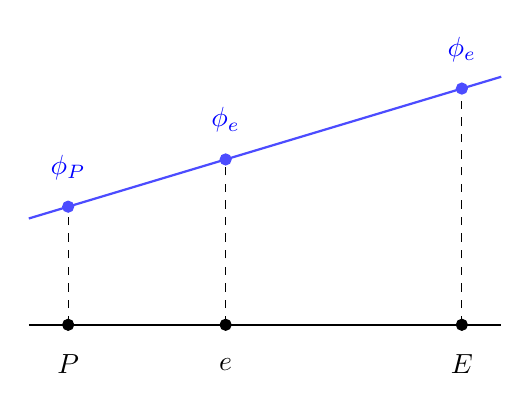
\begin{tikzpicture}
		% Ground
		\draw[thick] (0,0) -- ++(6,0);
		% Point P
		\filldraw[black] (0.5,0) circle (2pt);
		\draw[dashed] (0.5,0) -- ++(0,1.5);
		\node[black, yshift=-0.5cm] at (0.5,0) {$P$};
		\filldraw[blue!70!white] (0.5,1.5) circle (2pt);
		\node[blue, yshift=0.5cm] at (0.5,1.5) {$\phi_P$};
		% Point e
		\filldraw[black] (2.5,0) circle (2pt);
		\draw[dashed] (2.5,0) -- ++(0,{1.5+3/5});
		\node[black, yshift=-0.5cm] at (2.5,0) {$e$};
		\filldraw[blue!70!white] (2.5,{1.5+3/5}) circle (2pt);
		\node[blue, yshift=0.5cm] at (2.5,{1.5+3/5}) {$\phi_e$}; 
		% Point E
		\filldraw[black] (5.5,0) circle (2pt);
		\draw[dashed] (5.5,0) -- ++(0,3);
		\node[black, yshift=-0.5cm] at (5.5,0) {$E$};
		\filldraw[blue!70!white] (5.5,3) circle (2pt);
		\node[blue, yshift=0.5cm] at (5.5,3.0) {$\phi_e$}; 
		% Blue line
		\draw[thick, blue!70!white] (0,{1.5-1.5/10}) -- (6,{1.5+1.5*5.5/5});
	\end{tikzpicture}
	\caption{Central Difference Scheme (CDS)}
	\label{fig:central_difference_scheme}
\end{figure}

\noindent
Thereby $\phi_e$ can be obtained interpolating between $\phi_P$ and $\phi_E$,
\begin{equation}
	\phi_e - \phi_P = f_e \left( \phi_E - \phi_P \right), \quad f_e = \frac{d_{Pe}}{d_{PE}}
\end{equation}
This yields a $2^{\text{nd}}$ order approximation for $\phi_e$ if $d_{Pe} = d_{Ee}$. Indeed, applying Taylor's theorem about the point $x_e$ and using Lagrange's remainder,
\begin{equation} \label{eq:cds_taylor_expansion}
	\phi_P = 
	\phi_e 
	- \left(\pdv{\phi}{x}\right)_e d_{Pe} 
	+ \frac{1}{2} \left(\pdv[2]{\phi}{x}\right)_e d_{Pe}^2 
	+ \frac{1}{6} \left(\pdv[3]{\phi}{x}\right)_{\xi_1} d_{Pe}^3
\end{equation}
where $\xi_1$ is some point lying in the convex combination of $(x_P, y_P)$ and $(x_E, y_E) = (x_E, y_P)$, that is, a point contained in the set $\{ (\lambda x_E + (1 - \lambda) x_P, y_P) \mid \lambda \in (0,1) \}$. On the other hand, the $2^\text{nd}$ order approximation of the derivative $(\partial_x \phi)_e$ is given by
\begin{equation} \label{eq:cds_derivative_approximation}
	\left(\pdv{\phi}{x}\right)_e = 
	\frac{\phi_E - \phi_P}{d_{PE}} - \left(\pdv[3]{\phi}{x}\right)_{\xi_2} \frac{d_{PE}^2}{3!} = 	
	\frac{\phi_E - \phi_P}{d_{PE}} - \left(\pdv[3]{\phi}{x}\right)_{\xi_2} \frac{(d_{Pe} + d_{Ee})^2}{3!}
\end{equation}
where, again, $\xi_2$ is some point obtained as the convex combination of $(x_P, y_P)$ and $(x_E, y_E)$. Introducing \eqref{eq:cds_derivative_approximation} in \eqref{eq:cds_taylor_expansion} and imposing $d_{Pe} = d_{Ee}$, 
\begin{equation} \label{eq:cds_error_terms}
	\phi_e - \phi_P = 
	\frac{d_{Pe}}{d_{PE}} (\phi_E - \phi_P) - 
	\left( \pdv[2]{\phi}{x} \right)_e \frac{d_{Pe}^2}{2} -
	\left\{ 
	\left( \pdv[3]{\phi}{x} \right)_{\xi_1} + 4 \left( \pdv[3]{\phi}{x} \right)_{\xi_2}
	\right\} 
	\frac{d_{Pe}^3}{6}
\end{equation}
As CDS retains the first term on the left--hand side of \eqref{eq:cds_error_terms}, the highest order term of the error is $\frac{1}{2} (\partial_x^2 \phi)_e d_{Pe}^2$, proving that CDS provides a $2^\text{nd}$ order approximation of $\phi_e$ when $d_{Pe} = d_{Ee}$. Nonetheless, this scheme is prone to stability problems producing oscillatory problems since the approximation is of order higher than $1$.

\subsubsection{Quadratic Upwind Interpolation for Convective Kinematics (QUICK)}

A logical improvement of CDS is using a parabola to interpolate between nodal points rather than a straight line. To construct a parabola three points are needed. As aforementioned, upstream conditions have a greater influence on flow properties than downstream conditions for incompressible flows and low Mach number gases. QUICK scheme takes profit of this fact. In order to ease the study, some notation is introduced. Located at the face position, $D$ refers to the downstream node, $C$ is the first upstream node and $U$ is the most upstream node.

\begin{figure}[h]
	\centering
	\begin{minipage}{.5\textwidth}
		\centering
		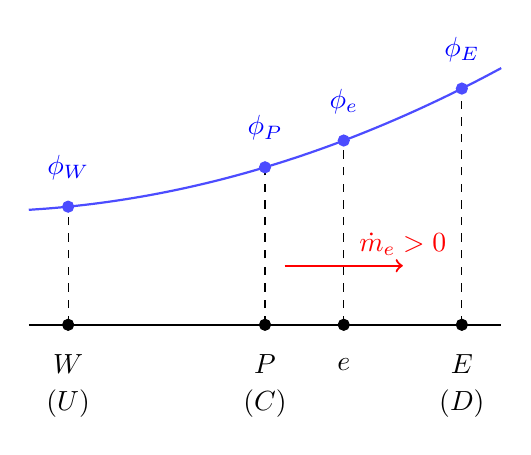
\begin{tikzpicture}
			% Points
			\def\zerox{0.5}
			\def\zeroy{1.5}
			\def\onex{3}
			\def\oney{2}
			\def\twox{5.5}
			\def\twoy{3}
			\def\coefa{1.5}
			\def\coefb{0.2}
			\def\coefc{0.04}
			% Ground
			\draw[thick] (0,0) -- ++(6,0);
			% Point W
			\filldraw[black] (\zerox,0) circle (2pt);
			\draw[dashed] (\zerox,0) -- ++(0,\zeroy);
			\node[black, yshift=-0.5cm] at (\zerox,0) {$W$};
			\node[black, yshift=-1cm] at (\zerox,0) {$(U)$};
			\filldraw[blue!70!white] (\zerox,\zeroy) circle (2pt);
			\node[blue, yshift=0.5cm] at (\zerox,\zeroy) {$\phi_W$};
			% Point P
			\filldraw[black] (\onex,0) circle (2pt);
			\draw[dashed] (\onex,0) -- ++(0,\oney);
			\node[black, yshift=-0.5cm] at (\onex,0) {$P$};
			\node[black, yshift=-1cm] at (\onex,0) {$(C)$};
			\filldraw[blue!70!white] (\onex,\oney) circle (2pt);
			\node[blue, yshift=0.5cm] at (\onex,\oney) {$\phi_P$};
			% Point e
			\filldraw[black] ({\onex+1},0) circle (2pt);
			\draw[dashed] ({\onex+1},0) -- ++(0,2.34);
			\node[black, yshift=-0.5cm] at ({\onex+1},0) {$e$};
			\filldraw[blue!70!white] ({\onex+1},2.34) circle (2pt);
			\node[blue, yshift=0.5cm] at ({\onex+1},2.34) {$\phi_e$};
			% Point E
			\filldraw[black] (\twox,0) circle (2pt);
			\draw[dashed] (\twox,0) -- ++(0,\twoy);
			\node[black, yshift=-0.5cm] at (\twox,0) {$E$};
			\node[black, yshift=-1cm] at (\twox,0) {$(D)$};
			\filldraw[blue!70!white] (\twox,\twoy) circle (2pt);
			\node[blue, yshift=0.5cm] at (\twox,\twoy) {$\phi_E$}; 
			% Blue line
			\draw[scale=1, domain=0:6, smooth, variable=\x, blue!70!white, thick] plot ({\x}, {\coefa + \coefb*(\x-\zerox) + \coefc*(\x-\zerox)*(\x-\onex)});
			% Mass flow
			\draw[->, red, thick] (3.25,0.75) -- ++(1.5,0) node[above]{$\dot{m}_e > 0$};
		\end{tikzpicture}
		\captionsetup{width=0.9\textwidth}
		\caption{QUICK when $(\vb{v} \vdot \vb{n})_e > 0$.}
		\label{fig:quick_1}
	\end{minipage}%
	\begin{minipage}{.5\textwidth}
		\centering
		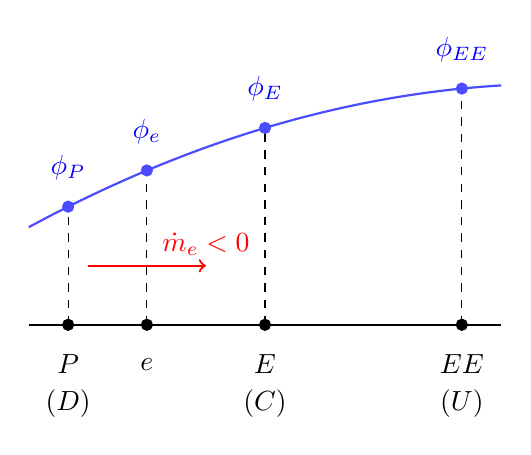
\begin{tikzpicture}
			% Points
			\def\zerox{0.5}
			\def\zeroy{1.5}
			\def\onex{3}
			\def\oney{2.5}
			\def\twox{5.5}
			\def\twoy{3}
			\def\coefa{1.5}
			\def\coefb{0.4}
			\def\coefc{-0.04}
			% Ground
			\draw[thick] (0,0) -- ++(6,0);
			% Point P
			\filldraw[black] (\zerox,0) circle (2pt);
			\draw[dashed] (\zerox,0) -- ++(0,\zeroy);
			\node[black, yshift=-0.5cm] at (\zerox,0) {$P$};
			\node[black, yshift=-1cm] at (\zerox,0) {$(D)$};
			\filldraw[blue!70!white] (\zerox,\zeroy) circle (2pt);
			\node[blue, yshift=0.5cm] at (\zerox,\zeroy) {$\phi_P$};
			% Point e
			\filldraw[black] ({\zerox+1},0) circle (2pt);
			\draw[dashed] ({\zerox+1},0) -- ++(0,1.96);
			\node[black, yshift=-0.5cm] at ({\zerox+1},0) {$e$};
			\filldraw[blue!70!white] ({\zerox+1},1.96) circle (2pt);
			\node[blue, yshift=0.5cm] at ({\zerox+1},1.96) {$\phi_e$};
			% Point e
			\filldraw[black] (\onex,0) circle (2pt);
			\draw[dashed] (\onex,0) -- ++(0,\oney);
			\node[black, yshift=-0.5cm] at (\onex,0) {$E$};
			\node[black, yshift=-1cm] at (\onex,0) {$(C)$};
			\filldraw[blue!70!white] (\onex,\oney) circle (2pt);
			\node[blue, yshift=0.5cm] at (\onex,\oney) {$\phi_E$}; 
			% Point ee
			\filldraw[black] (\twox,0) circle (2pt);
			\draw[dashed] (\twox,0) -- ++(0,\twoy);
			\node[black, yshift=-0.5cm] at (\twox,0) {$EE$};
			\node[black, yshift=-1cm] at (\twox,0) {$(U)$};
			\filldraw[blue!70!white] (\twox,\twoy) circle (2pt);
			\node[blue, yshift=0.5cm] at (\twox,\twoy) {$\phi_{EE}$}; 
			% Blue line
			\draw[scale=1, domain=0:6, smooth, variable=\x, blue!70!white, thick] plot ({\x}, {\coefa + \coefb*(\x-\zerox) + \coefc*(\x-\zerox)*(\x-\onex)});
			% Mass flow
			\draw[->, red, thick] (0.75,0.75) -- ++(1.5,0) node[above]{$\dot{m}_e < 0$};
		\end{tikzpicture}
		\captionsetup{width=0.9\textwidth}
		\caption{QUICK when $(\vb{v} \vdot \vb{n})_e < 0$.}
		\label{fig:quick_2}
	\end{minipage}
\end{figure}

\noindent
Let $(x_0, \phi_0)$, $(x_1, \phi_1)$, $(x_2, \phi_2)$ be the points which the polynomial $p(x)$ must interpolate, that is, $p(x_0) = \phi_0$, $p(x_1) = \phi_1$ and $p(x_2) = \phi_2$, satisfying $x_0 < x_1 < x_2$. If $(\vb{v} \vdot \vb{n})_e > 0$ then $x_0 = x_W$, $x_1 = x_P$ and $x_2 = x_E$, whereas $x_0 = x_P$, $x_1 = x_E$ and $x_2 = x_{EE}$ in case of $(\vb{v} \vdot \vb{n})_e < 0$. Let $p(x)$ be the following polynomial
\begin{equation}
	p(x) = a_0 + a_1 (x - x_0) + a_2 (x - x_0) (x - x_1), \quad a_0, a_1, a_2 \in \real
\end{equation}
Since the interpolating polynomial exists and is unique \colorbox{red}{referencia}, by imposing the interpolating condition, $p(x)$ will be the desired polynomial. The interpolating condition is,
\begin{equation}
	\left.
	\begin{aligned}
		p(x_0) &= a_0 = \phi_0 \\
		p(x_1) &= a_0 + a_1 (x_1 - x_0) = \phi_1 \\
		p(x_2) &= a_0 + a_1 (x_2 - x_0) + a_2 (x_2 - x_0) (x_2 - x_1) = \phi_2
	\end{aligned}	
	\right\}
\end{equation}
which yields the following linear system:
\begin{equation}
	\begin{pmatrix}
		1 & 0 & 0 \\
		1 & x_1 - x_0 & 0 \\
		1 & x_2 - x_0 & (x_2 - x_1)(x_2 - x_0)
	\end{pmatrix}
	\begin{pmatrix}
		a_0 \\ a_1 \\ a_2
	\end{pmatrix} = 
	\begin{pmatrix}
		\phi_0 \\ \phi_1 \\ \phi_2
	\end{pmatrix}
\end{equation}
The determinant of the system matrix is non-zero because the abscissae are distinct, therefore the system has a unique solution given by
\begin{equation}
	\left.
	\begin{aligned}
		a_0 &= \phi_0 \\
		a_1 &= \frac{\phi_1 - \phi_0}{x_1 - x_0} \\
		a_2 &= \frac{\phi_2 - \phi_0}{(x_2 - x_1)(x_2 - x_0)} - \frac{\phi_1 - \phi_0}{(x_2 - x_1)(x_1 - x_0)}
	\end{aligned}	
	\right\}
\end{equation}

\subsubsection{Second--order Upwind Linear Extrapolation (SUDS)}

\begin{figure}[h]
	\centering
	\begin{minipage}{.5\textwidth}
		\centering
		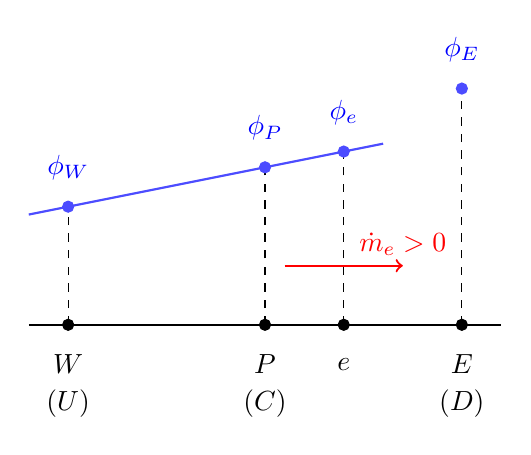
\begin{tikzpicture}
			% Points
			\def\zerox{0.5}
			\def\zeroy{1.5}
			\def\onex{3}
			\def\oney{2}
			\def\twox{5.5}
			\def\twoy{3}
			\def\coefa{1.5}
			\def\coefb{0.2}
			\def\coefc{0.04}
			% Ground
			\draw[thick] (0,0) -- ++(6,0);
			% Point W
			\filldraw[black] (\zerox,0) circle (2pt);
			\draw[dashed] (\zerox,0) -- ++(0,\zeroy);
			\node[black, yshift=-0.5cm] at (\zerox,0) {$W$};
			\node[black, yshift=-1cm] at (\zerox,0) {$(U)$};
			\filldraw[blue!70!white] (\zerox,\zeroy) circle (2pt);
			\node[blue, yshift=0.5cm] at (\zerox,\zeroy) {$\phi_W$};
			% Point P
			\filldraw[black] (\onex,0) circle (2pt);
			\draw[dashed] (\onex,0) -- ++(0,\oney);
			\node[black, yshift=-0.5cm] at (\onex,0) {$P$};
			\node[black, yshift=-1cm] at (\onex,0) {$(C)$};
			\filldraw[blue!70!white] (\onex,\oney) circle (2pt);
			\node[blue, yshift=0.5cm] at (\onex,\oney) {$\phi_P$};
			% Point e
			\filldraw[black] ({\onex+1},0) circle (2pt);
			\draw[dashed] ({\onex+1},0) -- ++(0,{1.5+0.5*3.5/2.5});
			\node[black, yshift=-0.5cm] at ({\onex+1},0) {$e$};
			\filldraw[blue!70!white] ({\onex+1},{1.5+0.5*3.5/2.5}) circle (2pt);
			\node[blue, yshift=0.5cm] at ({\onex+1},{1.5+0.5*3.5/2.5}) {$\phi_e$};
			% Point E
			\filldraw[black] (\twox,0) circle (2pt);
			\draw[dashed] (\twox,0) -- ++(0,\twoy);
			\node[black, yshift=-0.5cm] at (\twox,0) {$E$};
			\node[black, yshift=-1cm] at (\twox,0) {$(D)$};
			\filldraw[blue!70!white] (\twox,\twoy) circle (2pt);
			\node[blue, yshift=0.5cm] at (\twox,\twoy) {$\phi_E$}; 
			% Blue line
			\draw[scale=1, domain=0:4.5, smooth, variable=\x, blue!70!white, thick] plot ({\x}, {1.5+0.2*(\x-0.5)});
			% Mass flow
			\draw[->, red, thick] (3.25,0.75) -- ++(1.5,0) node[above]{$\dot{m}_e > 0$};
		\end{tikzpicture}
		\captionsetup{width=0.9\textwidth}
		\caption{SUDS when $(\vb{v} \vdot \vb{n})_e > 0$.}
		\label{fig:suds_1}
	\end{minipage}%
	\begin{minipage}{.5\textwidth}
		\centering
		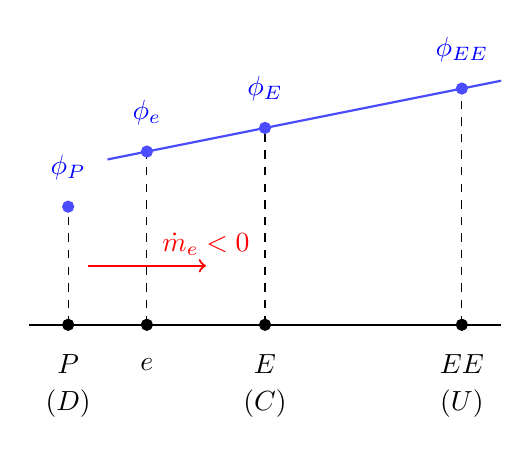
\begin{tikzpicture}
			% Points
			\def\zerox{0.5}
			\def\zeroy{1.5}
			\def\onex{3}
			\def\oney{2.5}
			\def\twox{5.5}
			\def\twoy{3}
			\def\coefa{1.5}
			\def\coefb{0.4}
			\def\coefc{-0.04}
			% Ground
			\draw[thick] (0,0) -- ++(6,0);
			% Point P
			\filldraw[black] (\zerox,0) circle (2pt);
			\draw[dashed] (\zerox,0) -- ++(0,\zeroy);
			\node[black, yshift=-0.5cm] at (\zerox,0) {$P$};
			\node[black, yshift=-1cm] at (\zerox,0) {$(D)$};
			\filldraw[blue!70!white] (\zerox,\zeroy) circle (2pt);
			\node[blue, yshift=0.5cm] at (\zerox,\zeroy) {$\phi_P$};
			% Point e
			\filldraw[black] ({\zerox+1},0) circle (2pt);
			\draw[dashed] ({\zerox+1},0) -- ++(0,{2.5-0.2*1.5});
			\node[black, yshift=-0.5cm] at ({\zerox+1},0) {$e$};
			\filldraw[blue!70!white] ({\zerox+1},{2.5-0.2*1.5}) circle (2pt);
			\node[blue, yshift=0.5cm] at ({\zerox+1},{2.5-0.2*1.5}) {$\phi_e$};
			% Point e
			\filldraw[black] (\onex,0) circle (2pt);
			\draw[dashed] (\onex,0) -- ++(0,\oney);
			\node[black, yshift=-0.5cm] at (\onex,0) {$E$};
			\node[black, yshift=-1cm] at (\onex,0) {$(C)$};
			\filldraw[blue!70!white] (\onex,\oney) circle (2pt);
			\node[blue, yshift=0.5cm] at (\onex,\oney) {$\phi_E$}; 
			% Point ee
			\filldraw[black] (\twox,0) circle (2pt);
			\draw[dashed] (\twox,0) -- ++(0,\twoy);
			\node[black, yshift=-0.5cm] at (\twox,0) {$EE$};
			\node[black, yshift=-1cm] at (\twox,0) {$(U)$};
			\filldraw[blue!70!white] (\twox,\twoy) circle (2pt);
			\node[blue, yshift=0.5cm] at (\twox,\twoy) {$\phi_{EE}$}; 
			% Blue line
			\draw[scale=1, domain=1:6, smooth, variable=\x, blue!70!white, thick] plot ({\x}, {2.5+0.2*(\x-3)});
			% Mass flow
			\draw[->, red, thick] (0.75,0.75) -- ++(1.5,0) node[above]{$\dot{m}_e < 0$};
		\end{tikzpicture}
		\captionsetup{width=0.9\textwidth}
		\caption{SUDS when $(\vb{v} \vdot \vb{n})_e < 0$.}
		\label{fig:suds_2}
	\end{minipage}
\end{figure}

\subsubsection{Exponential--Difference Scheme (EDS)}

The exponential difference scheme assumes a distribution for $\phi$ based on the steady 2--dimensional generalized convection--diffusion equation with no source term, that is to say,
\begin{equation}
	\frac{\dd}{\dd{x}} (\rho u \phi) = \frac{\dd}{\dd{x}} \left( \Gamma \frac{\dd{\phi}}{\dd{x}} \right)
\end{equation}
where $u$ is the component of $\vb{v}$ in the $x$ direction. So as to ease the study, $\rho u$ and $\Gamma$ are assumed to be constant. Thereby the initial value problem obtained is
\begin{equation} \label{eq:eds_ivp}
	\left\{
	\begin{aligned}
		&\frac{\dd^2 \phi}{\phi{x^2}} - \frac{\rho u}{\Gamma} \frac{\dd{\phi}}{\dd{x}} = 0 & &\text{in } (x_P, x_E) \\
		&\phi(x_P) = \phi_P \\
		&\phi(x_E) = \phi_E \\
	\end{aligned}
	\right.
\end{equation}
Problem \eqref{eq:eds_ivp} has existence and uniqueness of solution since it involves a linear ODE

\begin{equation}
	\phi(x) = 
	\phi_P - 
	\frac{\phi_E - \phi_P}{e^{\frac{\rho u}{\Gamma} d_{PE}} - 1} + 
	\frac{\phi_E - \phi_P}{e^{\frac{\rho u}{\Gamma} d_{PE}} - 1} e^{\frac{\rho u}{\Gamma} (x - x_P)}
\end{equation}

\subsubsection{Normalization of variables}

\subsubsection{Summary of schemes}